
%%% Uncomment for slide version
\documentclass{beamer}
\setbeameroption{hide notes} % Only slides

%%% Uncomment for handout version
%\documentclass[handout]{beamer}
%\setbeameroption{show notes on second screen=right} % Both

\usepackage{enumitem}
\usepackage{listings}
\usepackage{adjustbox} % To incorporate code into Latex
\usepackage{multirow} % To merge multiple rows  in a table
\usepackage{soul} % To put in strikethrough text
\usepackage{array}
\usepackage{makecell}

\setbeamertemplate{note page}{\pagecolor{white}\insertnote}
\setbeamertemplate{footline}{}
\usetheme[progressbar=frametitle]{moloch}% modern fork of the metropolis theme
\setbeamercolor{background canvas}{bg=white}
\setbeamercolor{progress bar}{use=palette primary,fg=black,bg=black}
\setbeamercolor{note page}{bg=white} 
\setbeamertemplate{date}{}


\DeclareUnicodeCharacter{0313}{*************************************}

\setbeamertemplate{page number in head/foot}{}


\addtobeamertemplate{navigation symbols}{}{%
	\usebeamerfont{footline}%
	\usebeamercolor[fg]{footline}%
	\hspace{1em}%
	\insertframenumber/\inserttotalframenumber
}
\setbeamercolor{itemize item}{fg=black}
\setbeamercolor{itemize subitem}{fg=black}
\setbeamercolor{itemize subsubitem}{fg=black}

\newcommand\blfootnote[1]{%
	\begingroup
	\renewcommand\thefootnote{}\footnote{#1}%
	\addtocounter{footnote}{-1}%
	\endgroup
}

%%%%%%%%%%%%%%%%%%
%%%%%%%%%%%%%%%%%%
%%%%%%%%%%%%%%%%%%
%%%%%%%%%%%%%%%%%%
%%%%%%%%%%%%%%%%%%
%%%%%%%%%%%%%%%%%%
%%%%%%%%%%%%%%%%%%




\title{\Huge FRST302: Forest Genetics}
\author{\Large Lecture 1.6: Identifying Genetic Variation }
\date{\today}

\begin{document}
	\maketitle
	
	\note{\emph{Remember, everything on the lecture slides and the accompanying notes is potentially examinable!}}
	% for the beamer version
	%\documentclass{beamer}
	
	\begin{frame}
		\frametitle{Lecture 1.5 - Recap}
		\begin{itemize}
			\item[--] Describe gene structure
			\item[--] The various roles of RNA
			\item[--] Describe gene expression
			\item[--] Identifying functional regions in a genome
			
		\end{itemize}
	\end{frame}
	
	
	
	\begin{frame}
		\frametitle{Terminology Check}
		\begin{itemize}
\item[]\textbf{Genome} - the complete set of genetic information for an organism
\item[]\textbf{Transcriptome} - the set of all RNA molecules, including mRNA, tRNA, and rRNA produced by the genome of an organism or a cell
\item[]\textbf{*Proteome} – the set of all proteins produced by an organism or a cell
\item[] \textbf{*Exome} - the subset of the genome that encodes for proteins
		
		\end{itemize}
		\blfootnote{* We haven't mentioned these up til now}
	\end{frame}
	
	
	
\begin{frame}
\frametitle{Learning Outcomes}
\begin{itemize}
	\item[--] The importance of genetic variation
	\item[--] Understand phenotypic variation and its connection to genetic variation
	\item[--] Different ways to study genetic variation
	\item[--] Single Nucleotide Polymorphisms (SNPs) - detection, use and limitations
\end{itemize}
\end{frame}
	
	
	


\begin{frame}
	\frametitle{The Importance of Variation}
	\centering 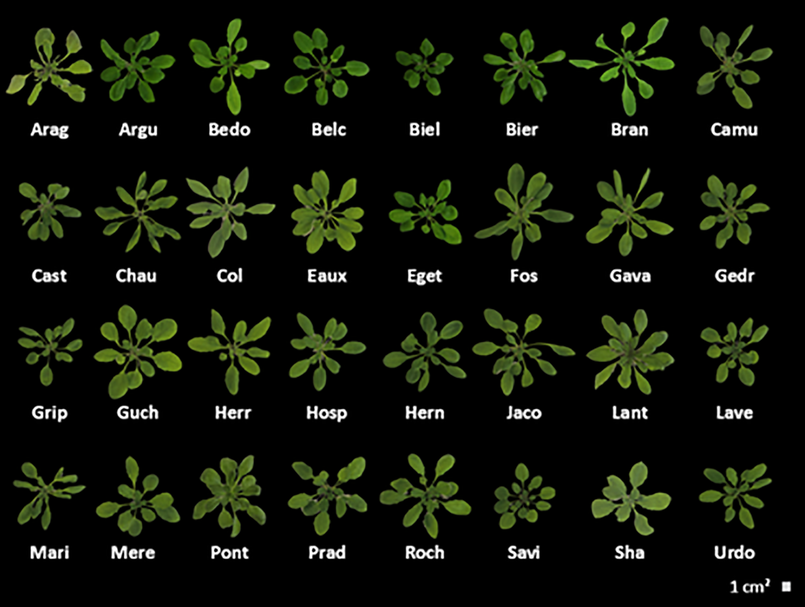
\includegraphics[keepaspectratio, width  = 0.8\textwidth]{img/arabidopsisVariation}\\
	\blfootnote{Variation in rosettes of \textit{Arabidopsis thaliana} individuals grown under controlled conditions in a growth chamber; Modified from Duruflé et al 2019 - \textit{Front Plant Sci.}}\\ 
\end{frame}						
			
\begin{frame}
\frametitle{The Importance of Variation}
\begin{columns}
	\begin{column}{0.5\textheight}
						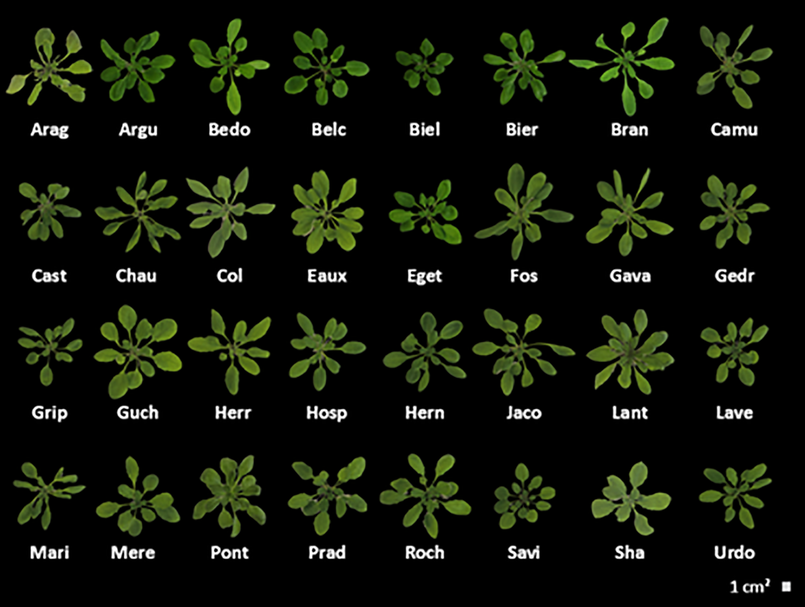
\includegraphics[keepaspectratio, width  = \textwidth]{img/arabidopsisVariation}
						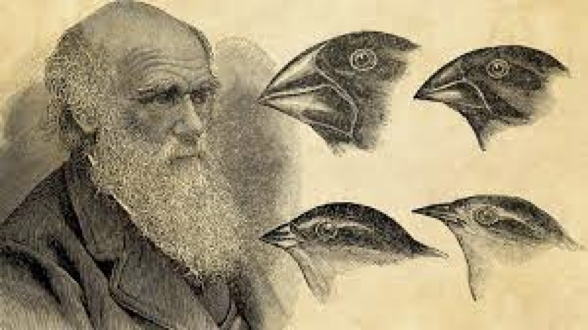
\includegraphics[keepaspectratio, width  = \textwidth]{img/DarwinFinch}
	\end{column}
	\begin{column}{0.5\textheight}
\begin{itemize}
	\item[--] Genetic variation is the foundation of evolution \pause
	\item[--] It predicts the response to selection and breeding \textsuperscript{\textit{Tongli will greatly expand on this}}\pause
	\item[--] Preservation of genetic diversity is a major goal of conservation
	\end{itemize}
	\end{column}
\end{columns}\pause 
\vspace{10pt}
\centering We can study genetic variation by examining patterns of phenotypic variation \\(e.g. within families - \textit{we've already done this}!) \\


\end{frame}




\begin{frame}
	
	\frametitle{Common Modes of Trait Variation}
	
		\textbf{Continuous} phenotypic variation - traits measured on a numerical scale (e.g. height, diameter, chlorophyll fluorescence) 
				\centering 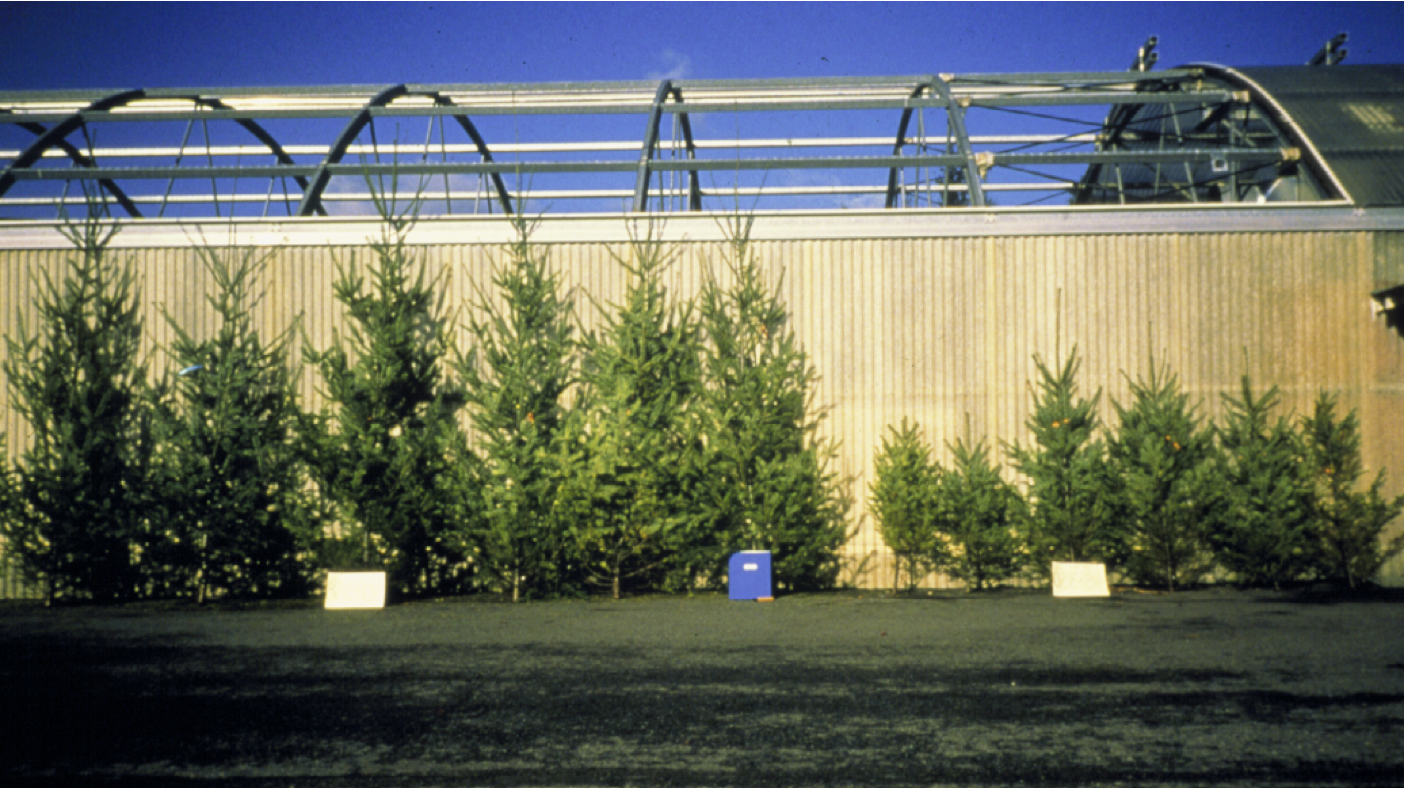
\includegraphics[keepaspectratio, width  = \textwidth]{img/treeVariation}\\

	
	
\blfootnote{These trees are from the same origin and were grown in the same environment!}
\end{frame}


\begin{frame}
	
	\frametitle{Common Modes of Trait Variation}

		\textbf{Discrete} phenotypic variation - traits that exhibit categorical differences \\
			\vspace{10pt}

		\centering 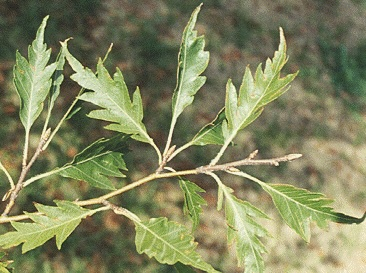
\includegraphics[keepaspectratio, width  = 0.4\textwidth]{img/cutBeechLeaf}\\
		\centering 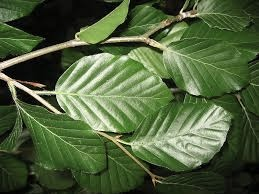
\includegraphics[keepaspectratio, width  = 0.4\textwidth]{img/roundBeechLeaf}\\
		
	
\end{frame}

\begin{frame}
	
	\frametitle{Common Modes of Trait Variation}
	
	\textbf{Ordinal} phenotypic variation - discrete traits with some informative order \\
	\vspace{10pt}
	
	\centering 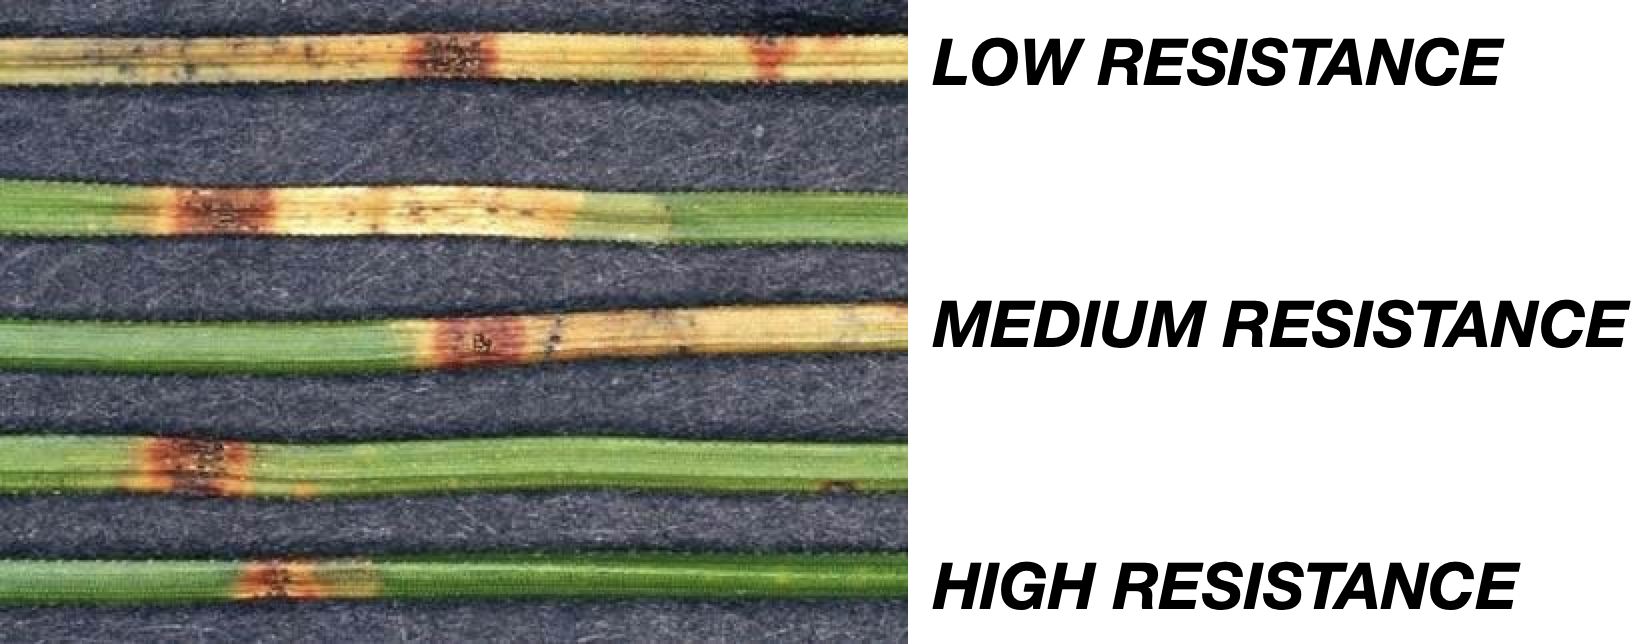
\includegraphics[keepaspectratio, width  = \textwidth]{img/dothistromaResistance}\\
	
	\blfootnote{Resistance to Dothistroma needle blight}
	
	
\end{frame}


\begin{frame}
	\frametitle{Difficulties Working With Phenotypes}
\textbf{	What are some difficulties you might face when using phenotypic variation to study genetic variation? \pause}
	\vspace{10pt}
	\begin{itemize}
		\item $Phenotype = Genotype + Environment$
		\item Different genotypes may express the same or similar phenotypes
		\item Phenotypic plasticity\textsuperscript{\textit{See the assigned reading!}}
		\item Time consuming
		\item Am I measuring the right thing? 
	\end{itemize}
	
	\pause
	\vspace{20pt}
\textit{	Directly working with genetic material is desirable!}
\end{frame}			


\begin{frame}
\frametitle{Now What!?}
\begin{columns}
	\begin{column}{0.5\textwidth}
		We've built a reference genome, we have identifed genes and gene regulatory regions\\
			\vspace{15pt}
						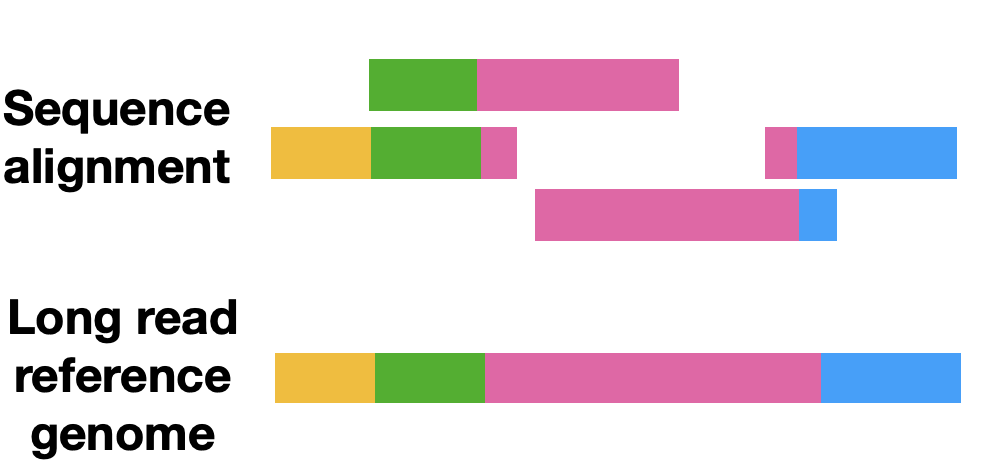
\includegraphics[keepaspectratio, width  = 0.7\textwidth]{img/referenceGenome}\\ 
			\vspace{15pt}
		How are we going to study genetic variation in our species of interest?
	\end{column}
	\begin{column}{0.5\textwidth}
	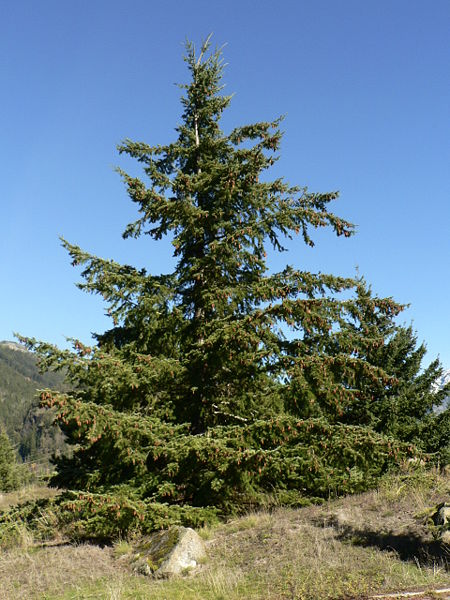
\includegraphics[keepaspectratio, width  = \textwidth]{img/doug-fir}\\ 
	\end{column}
\end{columns}
		
\end{frame}
	

	
\begin{frame}
		\frametitle{Types of Genetic Variation}
Based on what we've covered in the past lectures, how could we detect genetic variation? \\ \pause
	\vspace{10pt}

				\scriptsize
				\begin{itemize}
					\item[\textbf{1}] Differences in gene products (e.g. nonsynonymous point mutations)
					\item[\textbf{2}] Variation in RNA abundances (e.g. changes to the architechture of gene regulation)
					\item[\textbf{3}] Differences in genome structure (e.g. chromosomal rearrangements)
					\item[\textbf{4}] Differences in DNA sequences (e.g. nucleotide substitutions)
				\end{itemize}
				
				\blfootnote{\textit{This is \textbf{not} an exhaustive list!}}
		
	\end{frame}
	
	
	
	\begin{frame}
		\frametitle{1. Differences in Gene Products}
		
		
\centering				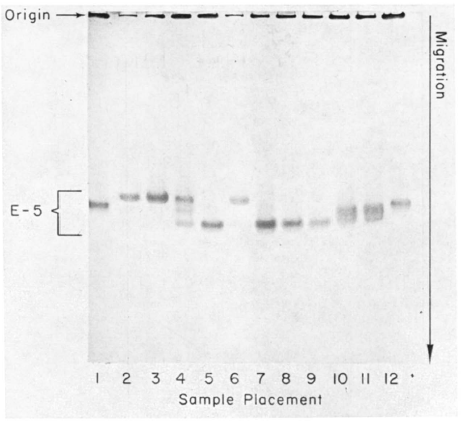
\includegraphics[keepaspectratio, width  = 0.7\textwidth]{img/LewontinHubby}
		
		\blfootnote{Figure from Lewontin and Hubby 1967 - \textit{Genetics} - One of the most important papers in genetic history!}
		
		
	\end{frame}





	\begin{frame}
		\frametitle{1. Differences in Gene Products}
		
		
		%%%
		\begin{columns}
			\begin{column}{0.5\textwidth}
				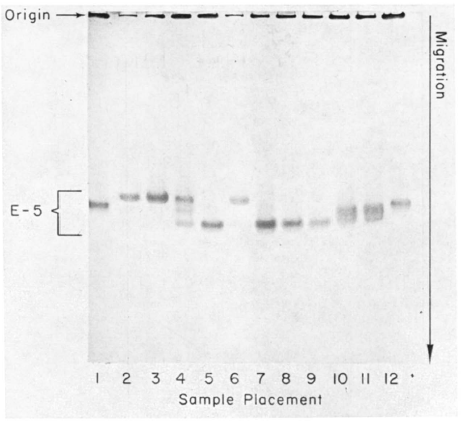
\includegraphics[keepaspectratio, width  = \textwidth]{img/LewontinHubby}
			\end{column}
			\begin{column}{0.5\textwidth}
				\begin{itemize}
					\item[$\bullet$] Extract specific enzymes and run them in starch gels
					\item[$\bullet$] Ectrophoretically polymorphic enzymes, or \textbf{allozymes}, separate on the gels
					\item[$\bullet$] Different alleles and genotypes can readily by seen from the gel itself
					\item[$\bullet$] Widely used from the 1970s-90s
				\end{itemize}
			\end{column}
		\end{columns}
		
		\blfootnote{Figure from Lewontin and Hubby 1967 - \textit{Genetics} - One of the most important papers in genetic history!}
		
		
	\end{frame}

	\begin{frame}
		\frametitle{Different Approaches}
		
		\centering 	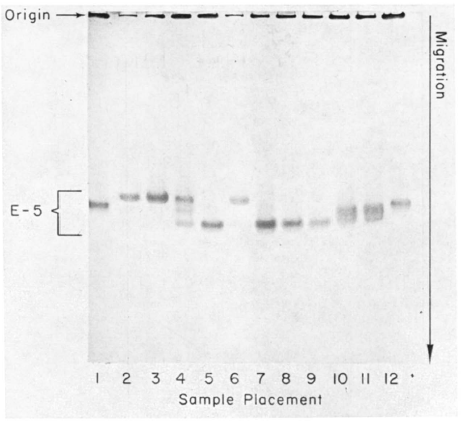
\includegraphics[keepaspectratio, width  = 0.3\textwidth]{img/LewontinHubby}\\
		\vspace{10pt}
		\centering \textbf{		\Large Allozymes }
		\vspace{10pt}
		\begin{columns}
			\begin{column}{0.5\textwidth}
				\centering			\underline{\textbf{Pros}}
				\begin{itemize}
					\item[$\bullet$] Easy sample prep
					\item[$\bullet$] No computation
					\item[$\bullet$] Cheap, no specialized equipment	
					\item[$\bullet$] ... 
				\end{itemize}
			\end{column}
			\begin{column}{0.5\textwidth}
				\centering			\underline{\textbf{Cons}}
				\begin{itemize}
					\item[$\bullet$] Hazardous - toxic chemicals
					\item[$\bullet$] Very low throughput
					\item[$\bullet$] ... 
				\end{itemize}
			\end{column}
			
			
		\end{columns}
		
		
	\end{frame}
	
	
\begin{frame}
		\frametitle{2. Variation in RNA Abundance}
\scriptsize
Differences in gene regulation are likely a major driver of phenotypic differences\\

\centering	\includegraphics[keepaspectratio, width  = 0.85\textwidth]{img/rna_seq}
\blfootnote{ In maize, \textit{$\approx$60\% of variation in agriculturally important traits can be linked to variation in gene regulation}}
\end{frame}
	

	\begin{frame}
		\frametitle{2. Variation in RNA Abundance}
\centering	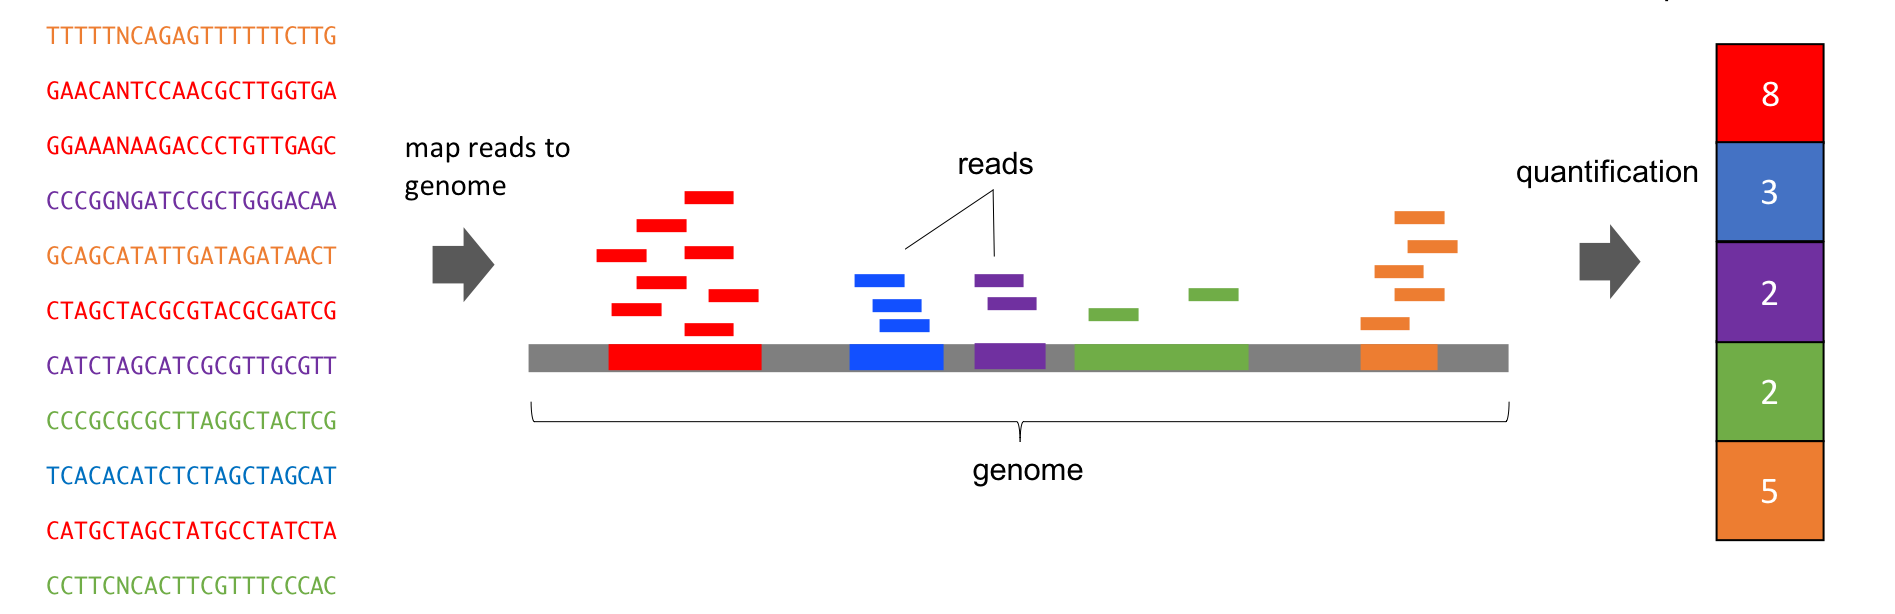
\includegraphics[keepaspectratio, width  = 0.9\textwidth]{img/rnaSeqSection}
\begin{columns}
	\begin{column}{0.5\textwidth}
					\centering	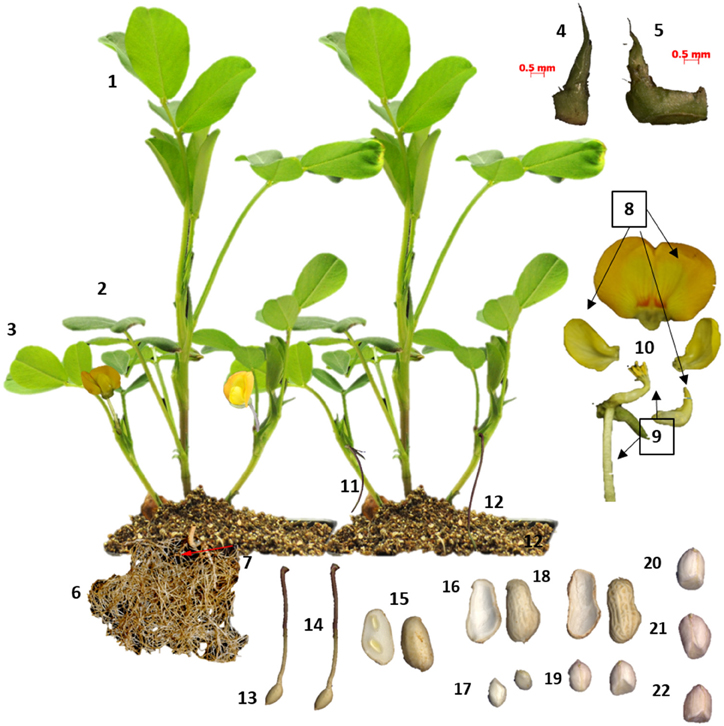
\includegraphics[keepaspectratio, width  = 0.8\textwidth]{img/peanut}	
					
					\end{column}
	\begin{column}{0.5\textwidth}
\scriptsize
	\begin{itemize}
		\item[$\bullet$] Compare expression of different transcripts among multiple individuals/populations
		\item[$\bullet$] Hypotheses regarding particular tissues and parts of the lifecycle can be devised and tested
		\item[$\bullet$] Genes/transcripts that show highly variable levels of expression may contribute to phenotypic differences
		
		\end{itemize}

	\end{column}
\end{columns}

\end{frame}




\begin{frame}
	\frametitle{Different Approaches}
	
	\centering 	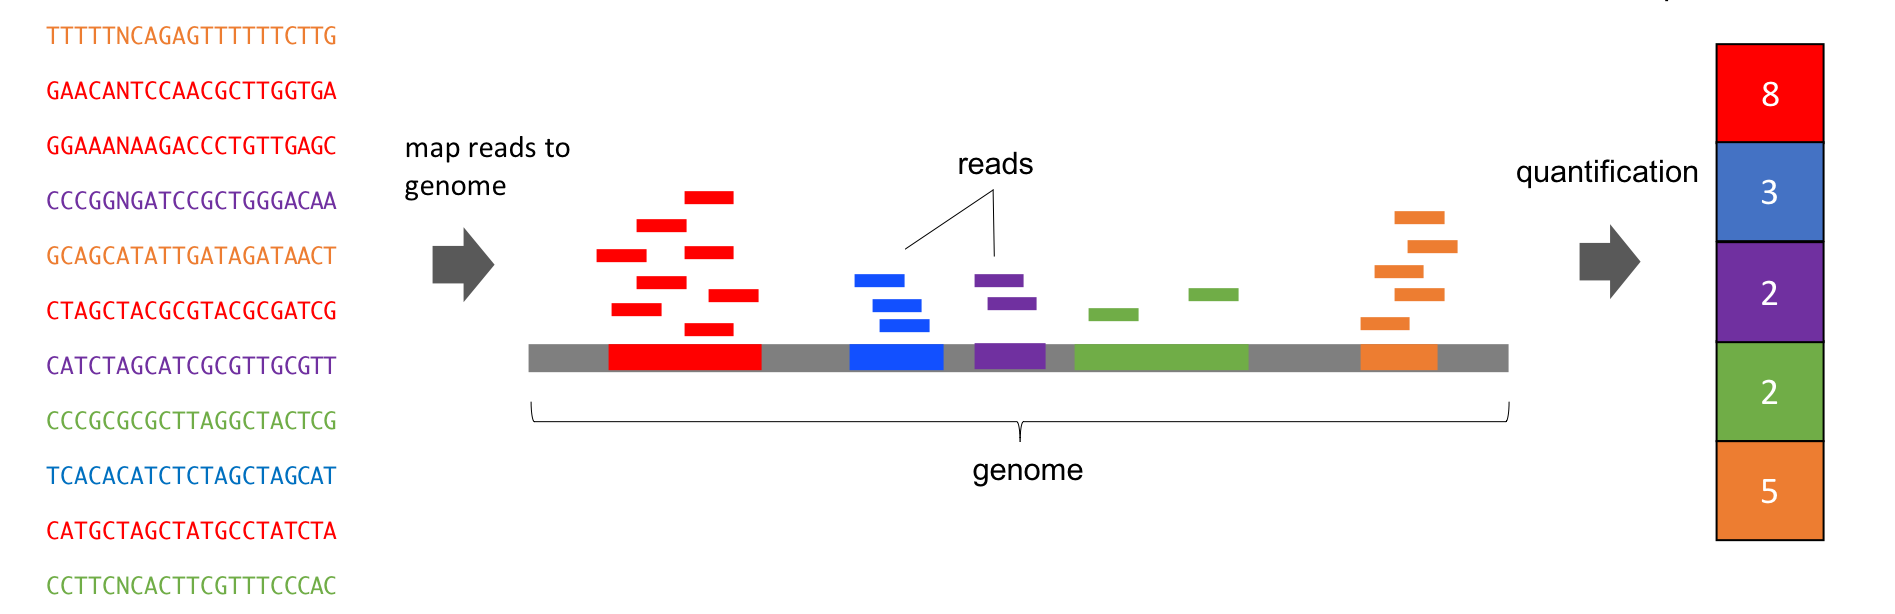
\includegraphics[keepaspectratio, width  = 0.8\textwidth]{img/rnaSeqSection}\\
	\vspace{10pt}
	\centering \textbf{		\Large Differentially Expressed Genes with RNA-Seq }
	\vspace{10pt}
	\begin{columns}
		\begin{column}{0.5\textwidth}
			\centering			\underline{\textbf{Pros}}
			\begin{itemize}
				\item[$\bullet$] Hypothesis driven
				\item[$\bullet$] Biologically interpretable
				\item[$\bullet$] Captures sequence variation too
				\item[$\bullet$] ... 
			\end{itemize}
		\end{column}
		\begin{column}{0.5\textwidth}
			\centering			\underline{\textbf{Cons}}
			\begin{itemize}
				\item[$\bullet$] Extremely large search space (e.g. tissues, life stages, environments)
				\item[$\bullet$] Statistically finicky
				\item[$\bullet$] ... 
			\end{itemize}
		\end{column}
		
		
	\end{columns}
\end{frame}



	
	
\begin{frame}
	\frametitle{3. Differences in Genome Structure}
	Variation in genome structure is \textit{relatively} common\\
	\vspace{5pt}
	Can range from large scale (differences in chromosome structure) to small scale (insertion/deletion of a single basepair)\\
		\vspace{5pt}
		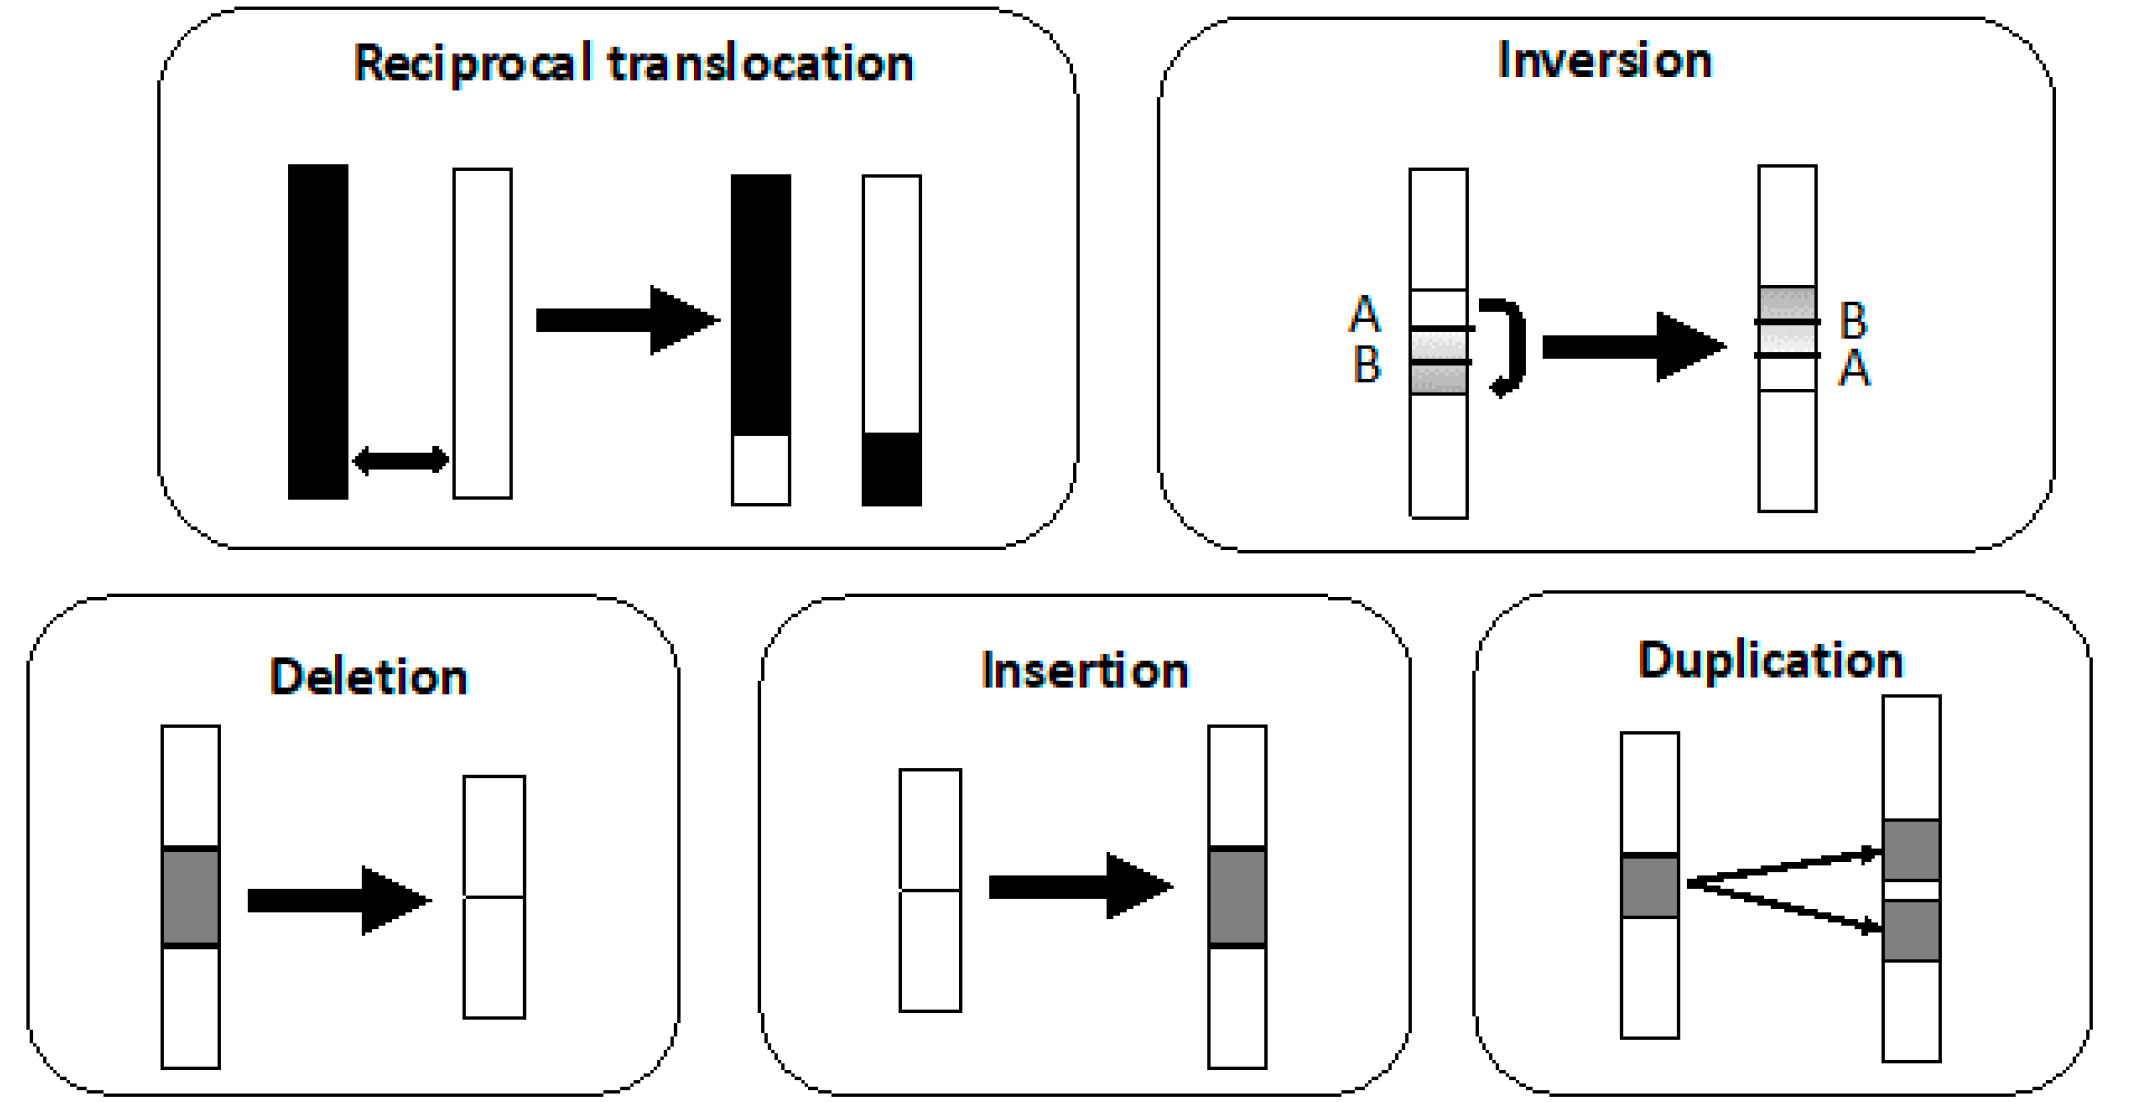
\includegraphics[keepaspectratio, width  = \textwidth]{img/structuralMutation}

\end{frame}

\begin{frame}
	\frametitle{3. Differences in Genome Structure}
Can be identifed by assembling and comparing whole genomes \\

	\vspace{5pt}

	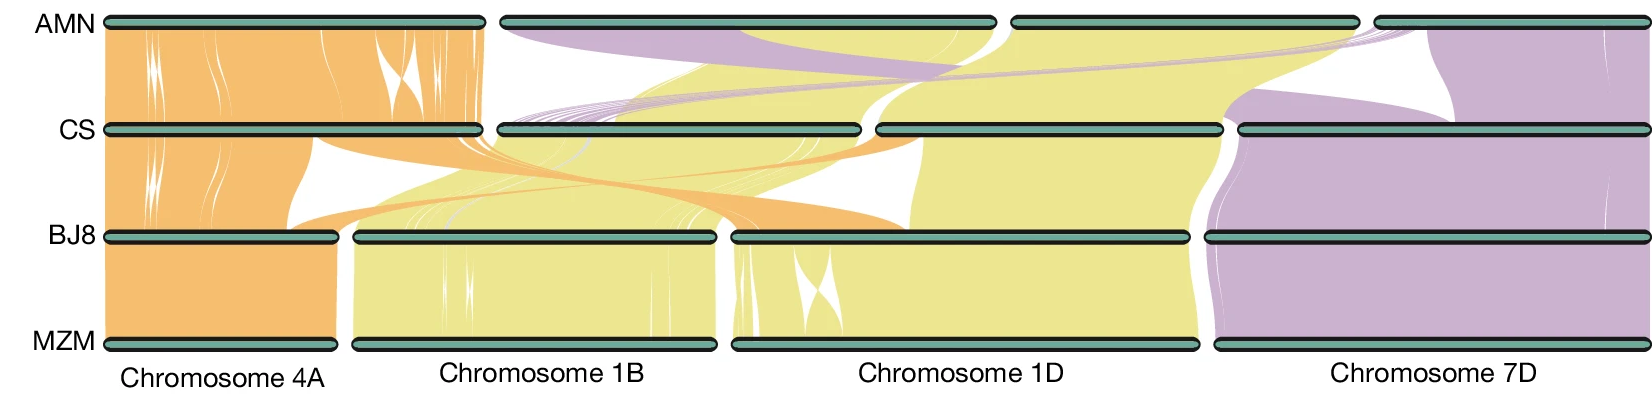
\includegraphics[keepaspectratio, width  = \textwidth]{img/wheatPangenome}\\ \pause
	\vspace{15pt}
\scriptsize	E.g. by assembling the genomes of 17 individuals of wheat, Jiao et al (2025 - Science) found $>$120,000 structural variants individually $>$5kbp - that's roughly 600Mbp of difference in genome structure \\
\vspace{10pt}
	\textit{Demonstrated that the development of Winter wheat was via gene duplication!}
	\blfootnote{Bread wheat is hexaploid with a genome size of $<$3Gbp}
	
\end{frame}
	


	
	\begin{frame}
		\frametitle{Different Approaches}
		
		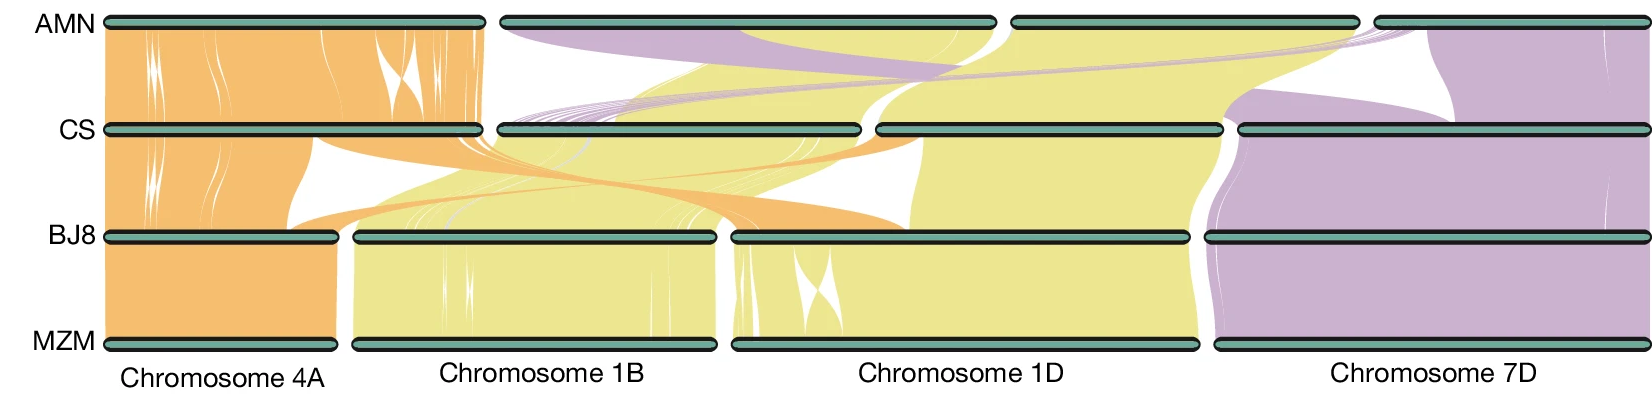
\includegraphics[keepaspectratio, width  = \textwidth]{img/wheatPangenome}\\
		\vspace{10pt}
		\centering \textbf{		\Large Assembling and comparing whole genomes}
		\vspace{10pt}
		\begin{columns}
			\begin{column}{0.5\textwidth}
				\centering			\underline{\textbf{Pros}}
				\begin{itemize}
					\item[$\bullet$] \textit{This is the future of genetics}
					\item[$\bullet$] Potentially identifies all genetic variation 
					\item[$\bullet$] Can get closer to causality
					\item[$\bullet$] ... 
				\end{itemize}
			\end{column}
			\begin{column}{0.5\textwidth}
				\centering			\underline{\textbf{Cons}}
				\begin{itemize}
					\item[$\bullet$] Currently prohibitively expensive
					\item[$\bullet$] Does not solve statistical inherent in genetic analysis
					\item[$\bullet$] Intense computation
					\item[$\bullet$] ... 
				\end{itemize}
			\end{column}
			
			
		\end{columns}
		
		
	\end{frame}
	

	
	
	\begin{frame}

		\Huge
		Questions? \\ \pause
		Let's take a short break
		
	\end{frame}
	



\begin{frame}
	\frametitle{Sample Exam Questions}
	\pause
	Under pure blending inheritance an individual’s trait is simply the arithmetic average of its parents trait values. By what fraction would you expect variation in that trait to decrease in the population each generation?
	
	\begin{itemize}
	\item [A] ...
	\item [B] ...
	\item [C] ...
	\item [D] ...
\end{itemize}
\end{frame}	

\begin{frame}
	\frametitle{Sample Exam Questions}
	
	Imagine Mendel had studied additional traits of his peas. Which of the following hypothetical traits would have made it difficult for him to formulate his laws:
	
	\begin{itemize}
		\item [A] ...
		\item [B] ...
		\item [C] ...
		\item [D] ...
	\end{itemize}
	
\end{frame}	

\begin{frame}
\Large 	4. Differences in DNA Sequences
\end{frame}


\begin{frame}
		
	\frametitle{Genetic Markers }

\begin{columns}
	\begin{column}{0.7\textwidth}
	A \textbf{genetic marker} is a gene$/$gene product or a DNA sequence that can be used to:
	\begin{itemize}
		\item[$\bullet$] Identify individuals or species
		\item[$\bullet$] Determine relationships among them
		\item[$\bullet$] Locate known genes 
		\item[$\bullet$] Study genetic variation

	\end{itemize} 

The development of genetic markers represents a major acheivement for biology in the 20th century

\end{column}
\begin{column}{0.3\textwidth}
	
\includegraphics[keepaspectratio, height  = 0.7\textheight]{img/geneticMarker}
\end{column}

\end{columns}

\end{frame}



\begin{frame}
	
	\frametitle{Genetic Markers }
	
	\begin{columns}
		\begin{column}{0.7\textwidth}
Desirable features of genetic markers:
			\begin{itemize}
				\item[$\bullet$] Easily distinguish hetero- and homozygotes
				\item[$\bullet$] HIghly polymorphic
				\item[$\bullet$] Reproducible/reliable 
				\item[$\bullet$] Distributed throughout the genome
				\item[$\bullet$] Fast and inexpensive
				\item[$\bullet$] Non-invasive/non-destructive collection of data
				
			\end{itemize} 
			

			
		\end{column}
		\begin{column}{0.3\textwidth}
			
\includegraphics[keepaspectratio, height  = 0.7\textheight]{img/geneticMarker}
		\end{column}
		
	\end{columns}
	
\end{frame}

\begin{frame}

\frametitle{Different Types of DNA Markers}

\begin{itemize}
	\item[$\bullet$] RFLP - Restriction Fragment Length Polymorphism 
	
	\item[$\bullet$] RAPD - Random Amplified Polymorphic DNA
	\item[$\bullet$] AFLP -  Amplified Fragment Length Polymorphism
	\item[] \textsuperscript{\textit{These have been largely superceded by DNA sequencing methods}}
	\vspace{20pt}
	\item[$\bullet$] SSR, Short Simple Repeats (also called Microsatellites)
	\item[] \textsuperscript{\textit{These are not really used in high throughput studies}}
	\vspace{20pt}
	\item[$\bullet$]  SNPs - Single Nucleotide Polymorphisms
	\item[] \textsuperscript{\textit{The sky is the limit!}}
\end{itemize}


\end{frame}






\begin{frame}
	
	\frametitle{Different Types of DNA Markers}
	
	\begin{itemize}
		\item[$\bullet$] RFLP - Restriction Fragment Length Polymorphism 
		
		\item[$\bullet$] RAPD - Random Amplified Polymorphic DNA
		\item[$\bullet$] AFLP -  Amplified Fragment Length Polymorphism
		
	\end{itemize}
	\vspace{15pt}
	All these methods involve examining the patterns of variation observed on gels (i.e. not high throughput) \\
	The data that arises from these methods can be hard to relate to phenotypes \\
	
	\vspace{20pt}
	
	Now that DNA sequencing is so cheap, these are kind of obsolete in forest genetics
\end{frame}





\begin{frame}
	
	\frametitle{Different Types of DNA Markers - Short Simple Repeats}
	
\begin{columns}
	\begin{column}{0.5\textwidth}
		\begin{itemize}
			\item[$\bullet$] SSRs – also called microsatellites or short tandem repeats (STRs)
			\item[$\bullet$] Usually about 1-10 bps
			\item[$\bullet$] Distributed at thousands of locations over the genome
			\item[$\bullet$] High mutation rates (so very polymorphic)
		\end{itemize}
		\end{column}
		\begin{column}{0.5\textwidth}
			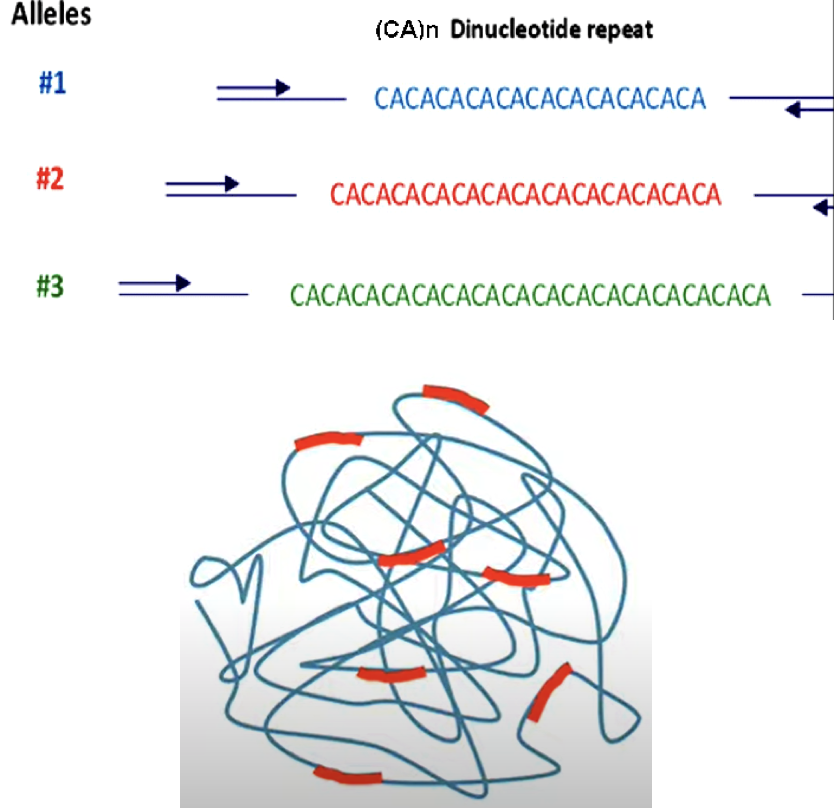
\includegraphics[keepaspectratio, width  = \textwidth]{img/microsat}
		\end{column}
	\end{columns}

\end{frame}



\begin{frame}
	
	\frametitle{Different Types of DNA Markers - Short Simple Repeats}
	
	\begin{columns}
		\begin{column}{0.5\textwidth}
			\textbf{Cons}
			\begin{itemize}
				\item[$\bullet$] Requires specific primers for target species
				\item[$\bullet$] Primer design is labour intensive
				\item[$\bullet$] Null alleles - if primer fails to bind a sample can appear homozygous

			\end{itemize}
		\end{column}
		\begin{column}{0.5\textwidth}
			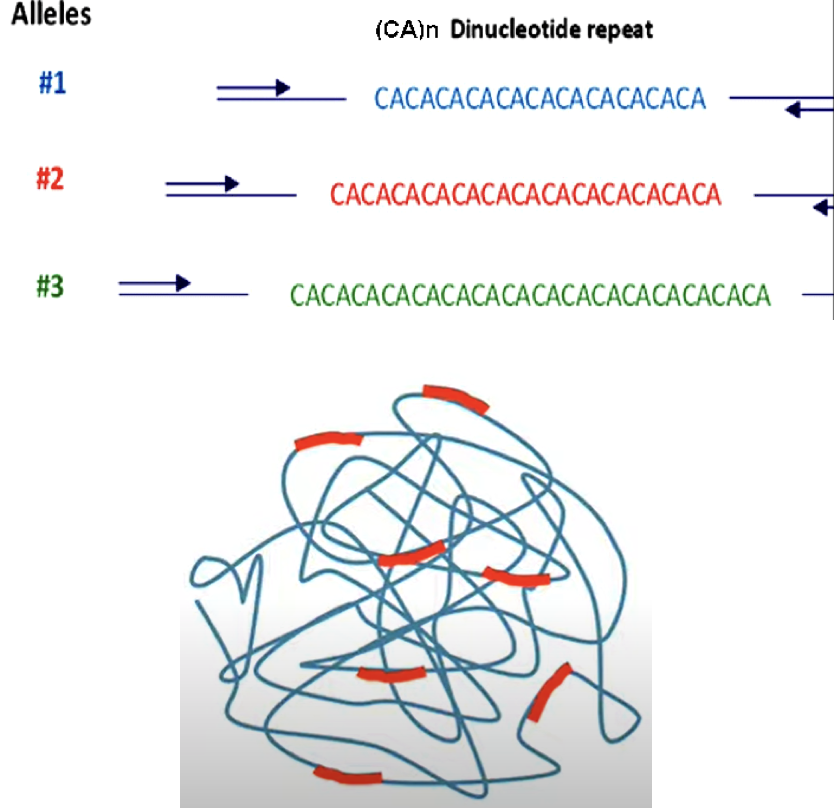
\includegraphics[keepaspectratio, width  = \textwidth]{img/microsat}
		\end{column}
	\end{columns}
	
	\vspace{15pt}
		Now that DNA sequencing is so cheap, these are less widely used than previously, but still useful in non-model systems
\end{frame}

\begin{frame}
	\frametitle{Single Nucleotide Polymorphism}
	A SNP (we often pronounce it as \textit{snip}) is a DNA polymorphism at a particular base pair in the genome\\
		\centering		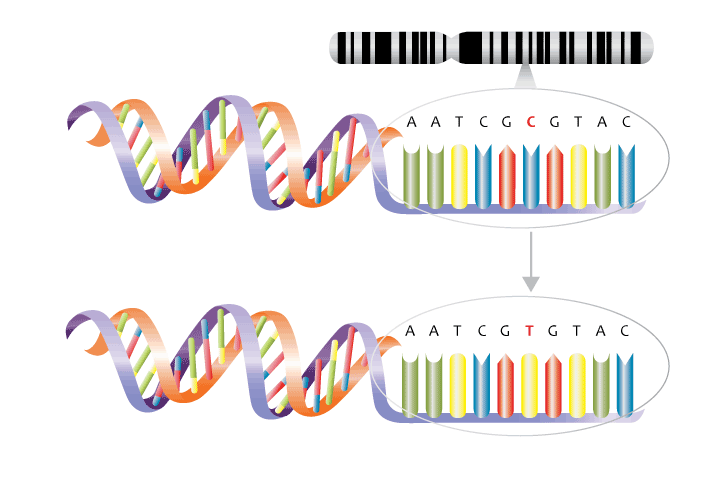
\includegraphics[keepaspectratio, width  = 0.7\textwidth]{img/SNP}
\end{frame}


\begin{frame}
	\frametitle{Identifying SNPs}
\Large How can we identify SNPs? \pause
	\centering		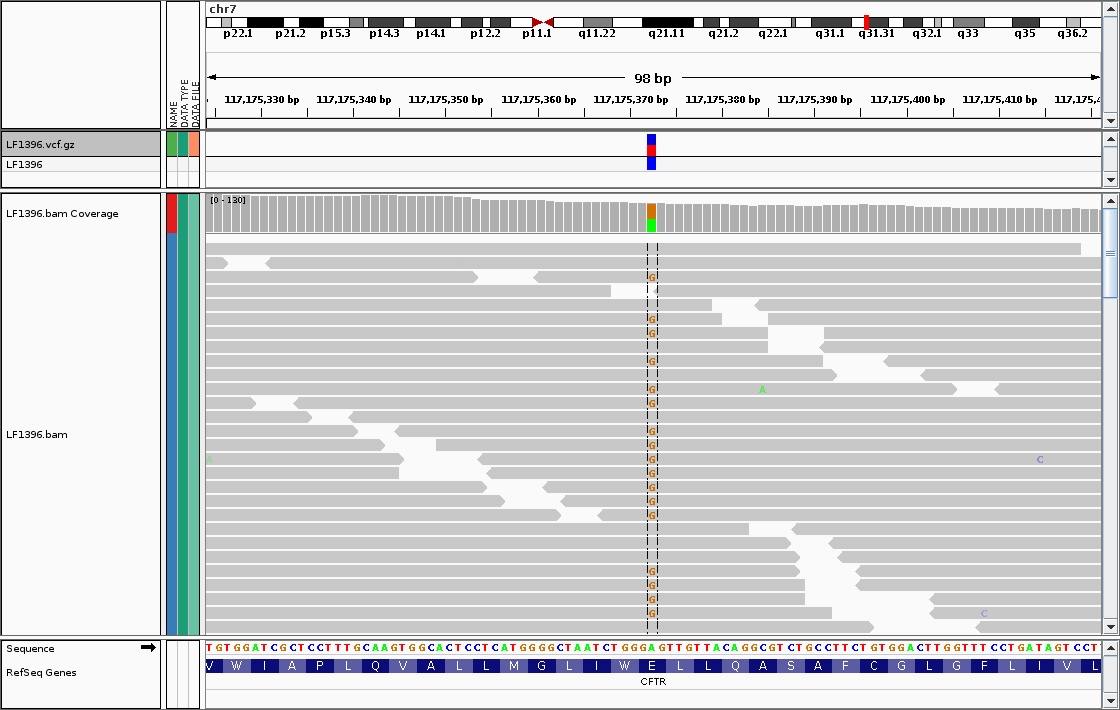
\includegraphics[keepaspectratio, width  = \textwidth]{img/IGV}
\end{frame}


\begin{frame}
	\frametitle{Identifying SNPs}

\centering How can we identify SNPs?\\

\vspace{20pt}

	\begin{columns}
	\begin{column}{0.5\textwidth}

		\begin{itemize}
			\item[$\bullet$] The first copy of the genome sequence can serve as a reference
			\item[$\bullet$] The fragment sequences from a new individual are compared to the reference to determine SNPs
			\item[$\bullet$] Technical error can also cause  false SNPs, then multiple reads are required to remove errors

		\end{itemize}
	\end{column}
	\begin{column}{0.5\textwidth}
		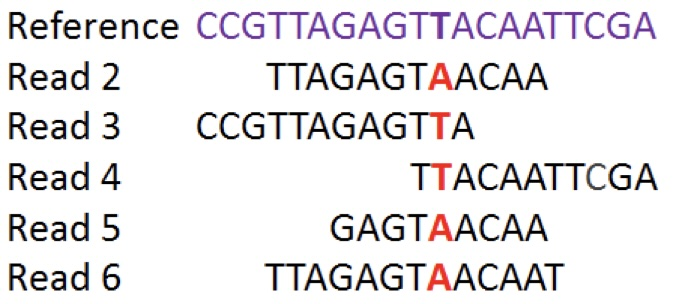
\includegraphics[keepaspectratio, width  = \textwidth]{img/readDiagram}
\end{column}
\end{columns}
\vspace{10pt}
\centering \textit{Repeat for as many individuals as you need/can afford!}
\end{frame}

\begin{frame}
	\frametitle{Genome Re-sequencing}
	
	We usually refer to the sequencing individuals after building a reference genome as \textbf{resequencing}\\
\vspace{5pt}
	There are many, many different ways to prepare the DNA for resequencing (we'll touch on these in Module 4)\\
\vspace{5pt}
	All high-throughput methods require the user to think about \textbf{sequencing coverage}\\
\vspace{5pt}
			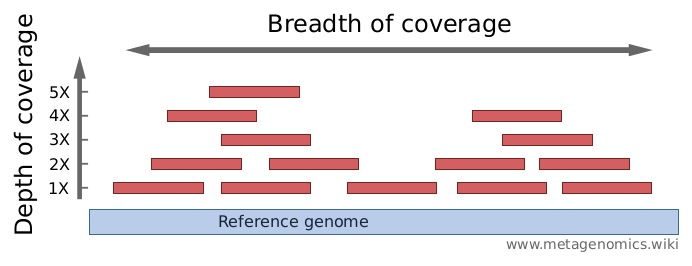
\includegraphics[keepaspectratio, width  = \textwidth]{img/depthBreadth}
	
	
\end{frame}

\begin{frame}
\frametitle{SNPs as Markers}
\begin{itemize}
	\item There can never be more than 4 alleles (i.e. A, T, C or G)
	\item Most SNPs only exhibit rwo alleles
		\item SNPs occur throughout the genome
		\item Easy to build statistical models to study them and relate them to phenotypes
		\item SNPs occur throughout the genome
		
\end{itemize}
\end{frame}


\begin{frame}
	\frametitle{Different Approaches}
	
	\centering 	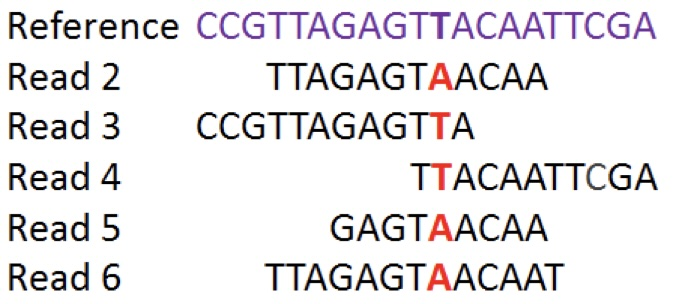
\includegraphics[keepaspectratio, width  = 0.4\textwidth]{img/readDiagram}\\
	\vspace{10pt}
	\centering \textbf{		\Large SNPs }
	\vspace{10pt}
	\begin{columns}
		\begin{column}{0.5\textwidth}
			\centering			\underline{\textbf{Pros}}
			\begin{itemize}
				\item[$\bullet$] Easy to model them statistically
				\item[$\bullet$] Millions of them in typical eukaryotic genomes (often found at around 0.1\% of sites)
				\item[$\bullet$] ... 
			\end{itemize}
		\end{column}
		\begin{column}{0.5\textwidth}
			\centering			\underline{\textbf{Cons}}
			\begin{itemize}
				\item[$\bullet$] Lots of computation /bioinformatics to identify them
				\item[$\bullet$] Hard to link to function in many cases
				\item[$\bullet$] Many statistical issues
				\item[$\bullet$] ... 
			\end{itemize}
		\end{column}
	\end{columns}
	
	\blfootnote{Analysis of SNPs is now a cornerstone of modern genomics (\textit{not just in trees!})}
\end{frame}




\begin{frame}
	\frametitle{Types of Genetic Variation}
Remember all the different things that we may use genomics for in forestry? Think about how you could tackle them with the different techniques we have discussed today.
\vspace{20pt}
	\scriptsize
	\begin{itemize}
		\item[\textbf{1}] Differences in gene products (identified with allozymes)
		\item[\textbf{2}] Variation in RNA abundances (identified with RNA-seq)
		\item[\textbf{3}] Differences in genome structure (identified with whole genome alignments)
		\item[\textbf{4}] Differences in DNA sequences (identified by fragment analysis or re-sequencing)
	\end{itemize}
	
	\blfootnote{\textit{This is \textbf{not} an exhaustive list!}}
	
\end{frame}



\begin{frame}

	\Huge
	Questions? \\ \pause
	Let's take a short break
	
\end{frame}

\begin{frame}
	\frametitle{Using Genetic Markers}
\scriptsize 
\begin{itemize}	
	\item[$\bullet$] We may be interested in identifying the genetic basis of an important trait\\
	\item[$\bullet$]  By looking for SNPs that have a particularly strong association with trait variation we may find important genes (e.g. targets for transformation etc.)
	\vspace{15pt} \pause
	\item[$\bullet$] Wang et al (2018 - Genome Biology) conducted a \textbf{genome-wide association study} (GWAS) to identify the genetic basis of adaptation to photoperiod in European Aspen (\textit{Populus tremula}) 
	\item \textit{They analysed $>4 million$ SNPs } \pause
 	\end{itemize}
	
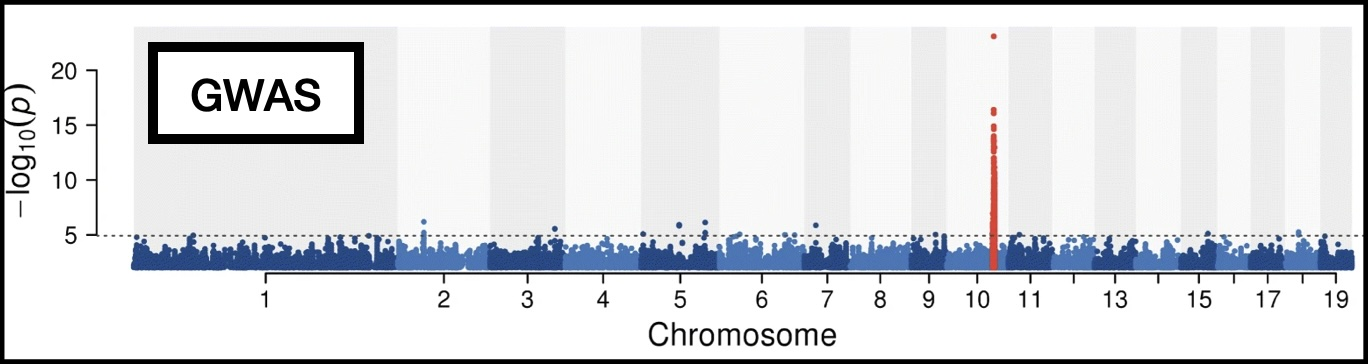
\includegraphics[keepaspectratio, width  = \textwidth]{img/gwas}

\textit{The genomic region highlighted by the red peak includes a gene that controls flowering time} \pause\\
BUT, there were more than 900 SNPs identified in the read peak that includes several different genes
\end{frame}



\begin{frame}
	\frametitle{Statistical Issues in Genetic Analysis}
	\textit{There is much more that can be said that would fit in a single course, let alone a lecture slide, so we'll return to this in Module 4}\\
	\vspace{30pt}
	For the time being, consider the following issues with genetic analysis:
\begin{itemize}
 \item[$\bullet$]		Correlation $\neq$ Causation
 \item[$\bullet$] 		Small effect loci require extremely large samples to adequately analyse
 \item[$\bullet$] 		Linkage and Linkage Disequilibrium
 \end{itemize}


 \end{frame}

\begin{frame}
	\frametitle{Linkage Disequilibrium}
\scriptsize 
	Due to genetic linkage, sites in close proximity on chromosomes will often be inherited together\\
	This generates a statistical relationship between the patterns of variation seen at different sites in the genome\\
	We use the term \textbf{linkage disequilibrium} to refer to non-random associations of alleles at two or more loci
	
				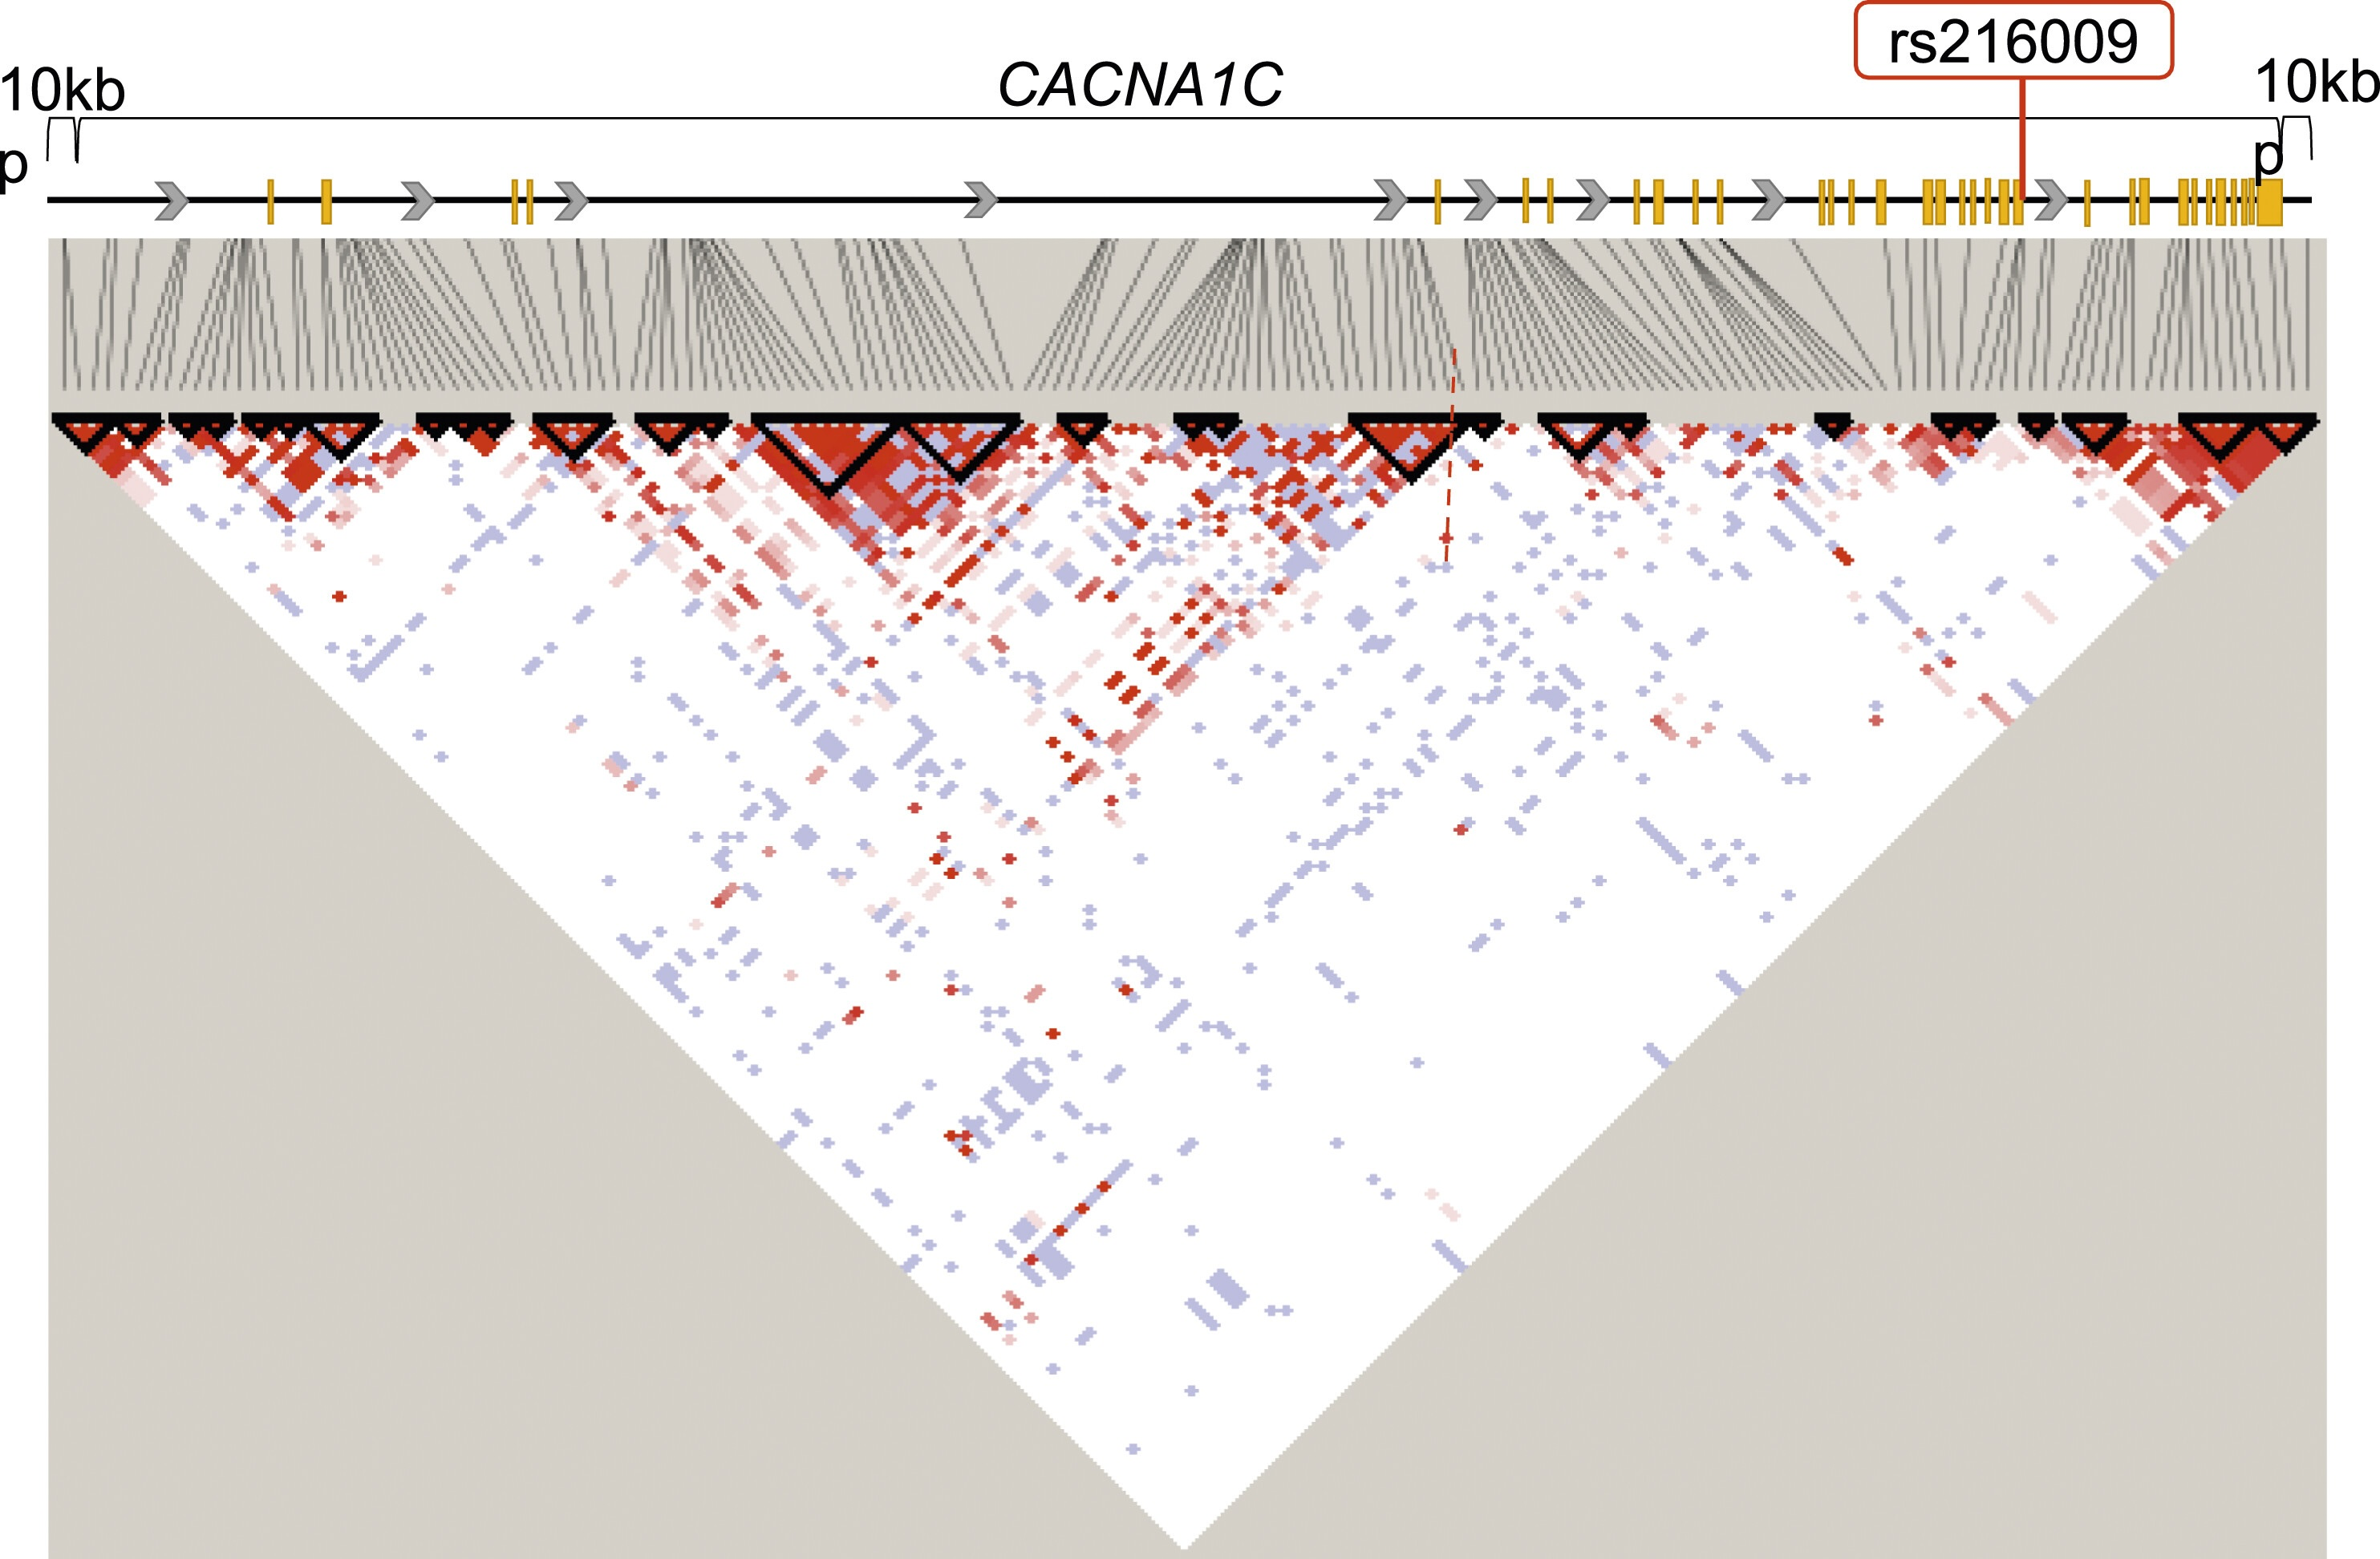
\includegraphics[keepaspectratio, width  = 0.8\textwidth]{img/LD_heat}\\

\vspace{10pt}
LD Introduces statistical non-independence into our analyses that we need to think about carefully!	
\end{frame}


\begin{frame}
	\frametitle{Learning Outcomes}
	\begin{itemize}
	\item[--] The importance of genetic variation
\item[--] Understand phenotypic variation and its connection to genetic variation
\item[--] Different ways to study genetic variation
\item[--] Single Nucleotide Polymorphisms (SNPs) - detection, use and limitations
	\end{itemize}
\end{frame}

\begin{frame}
\frametitle{Module Test 1}

\begin{itemize}
	\item \textbf{Don't prioritize memorization}
	\item Most questions will not test rote learning
\end{itemize}
\vspace{10pt}
				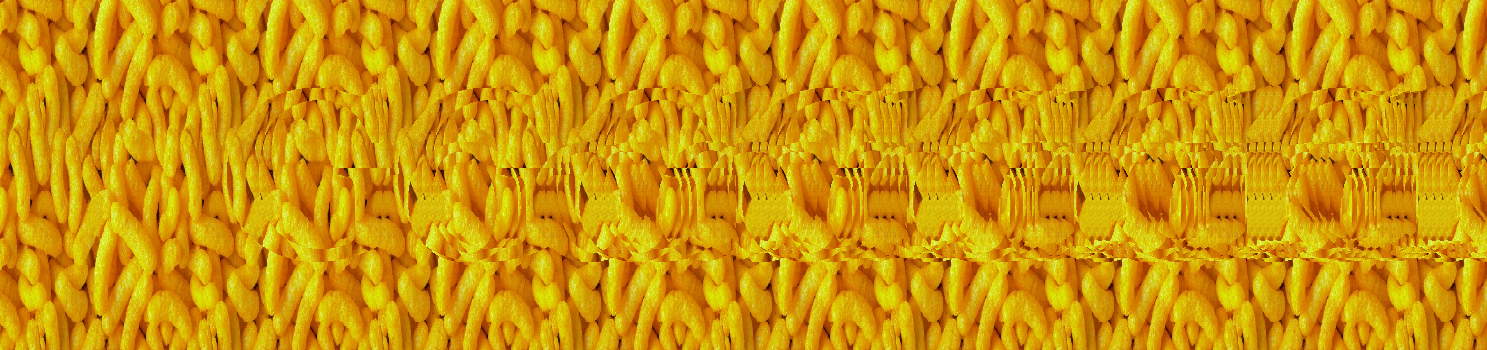
\includegraphics[keepaspectratio, width  = \textwidth]{img/magicEye}\\
\vspace{10pt}
\centering \textit{See you for the Module 1 review in a couple of weeks!}

\end{frame}


\end{document}



%%%
	\begin{columns}
	\begin{column}{0.5\textwidth}
	\end{column}
	\begin{column}{0.5\textwidth}
	\end{column}
\end{columns}



